%%%%%%%%%%%%%%%%%%%%%%%%%%%%%%%%%%%%%%%%%%%%%
%                Rubens Braz                %
%            www.rubensbraz.com             %
%                                           %
%         Para atualizações, checar:        %
%  https://github.com/rubensbraz/rel_latex  %
%                                           %
%   'Uma ratazana de esgoto sempre ajuda    %
%        outra ratazana de esgoto'.         %
%%%%%%%%%%%%%%%%%%%%%%%%%%%%%%%%%%%%%%%%%%%%%

% Definições Iniciais --------------------------------------------------
\documentclass[10pt, final, a4paper]{IEEEtran} % modelo do documento

\usepackage[pdftex]{graphicx} % exporta em PDF

\usepackage[portuguese]{babel} % tradução do documento

\usepackage[utf8]{inputenc} 
\usepackage[T1]{fontenc} % permite o uso de caracteres com acento 

\usepackage{url}
\usepackage[hidelinks]{hyperref} % exibição de links

\usepackage{hyphenat} % hífens

\usepackage{placeins} % controle de floats

\usepackage{etoolbox}
\apptocmd{\sloppy}{\hbadness 10000\relax}{}{} % remove erros de underfull hbox em links

\usepackage{color} % permite a mudança de cor do texto

\usepackage{xcolor,soul,framed}
\colorlet{shadecolor}{yellow} % define cor do destacado como amarelo

\usepackage{silence}
\WarningFilter{caption}{Unsupported document class} % remove o erro no pacote 'caption'
\usepackage{caption} % permite a inserção de legendas em imagens

\graphicspath{{../pdf/}{../jpeg/}}
\DeclareGraphicsExtensions{.pdf,.jpeg,.png} % formatos aceitos

\usepackage{array} 
\usepackage{mdwmath}
\usepackage{mdwtab} % tabelas

\usepackage{eqparbox} % facilita a criação de grupos

\usepackage{listings} % permite a escrita de códigos de programação

\renewcommand\thesection{\arabic{section}} % substitui os números romanos das seções por algarismos arábicos

\usepackage[cmex10]{amsmath}
\usepackage{amssymb}
\usepackage{mathtools} % fórmulas e símbolos matemáticos

\lstset{language=Matlab,%
	%basicstyle=\color{red},
	breaklines=true,%
	morekeywords={matlab2tikz},
	keywordstyle=\color{blue},%
	morekeywords=[2]{1}, keywordstyle=[2]{\color{black}},
	identifierstyle=\color{black},%
	stringstyle=\color{mylilas},
	commentstyle=\color{mygreen},%
	showstringspaces=false,%without this there will be a symbol in the places where there is a space
	numbers=left,%
	numberstyle={\tiny \color{black}},% size of the numbers
	numbersep=9pt, % this defines how far the numbers are from the text
	emph=[1]{for,end,break},emphstyle=[1]\color{red}, %some words to emphasise
	%emph=[2]{word1,word2}, emphstyle=[2]{style},
} % define modelo de exibição da linguagem Matlab

% Início do documento --------------------------------------------------
\begin{document}

\bstctlcite{IEEEexample:BSTcontrol}
	\title{Experiência Nº 1: Circuitos com diodos}
	\author{
		Rubens S. Braz Filho - 16/0144345\\
		Matheus Costa de Oliveira - 17/0019039\\
		Departamento de Engenharia Elétrica - ENE\\
		Universidade de Brasília - UnB
	}
\maketitle

% Resumo
\begin{abstract}
 Nesse relatório, as experiências laboratoriais e seus resultados serão apresentadas sequencialmente a seguir; a fonte usada nelas foi $v(t)=10sin(120 \pi t)$.\\
 Logo após as experiências, serão respondidas as questões experimentais e discussões.\\
 Adotamos os seguintes padrões de cores para os gráficos em função do tempo: tensão da fonte em amarelo; tensão medida em verde e em vermelho temos a tensão medida caso os diodos dos circuitos fossem ideais.
\end{abstract}

% Material necessário
\section{Material necessário}
\vspace{0.2cm}

\begin{itemize}
	\item 2 diodos 1N4007;
	
	\item 2 diodos Zener BZX75C2V4 ou equivalente;
	
	\item 1 resistor 1 k$\Omega$ / 0,25W;
	
	\item Equipamentos: osciloscópio de dois canais, gerador de sinais.
\end{itemize}
\FloatBarrier

\section*{Experiências Laboratoriais:}
\vspace{0.5cm}

% Experiência 1
\section{Experiência 1}

O circuito montado no laboratório para a experiência 1 é mostrado na figura \ref{ca}.

\begin{figure}[ht!]
	\captionsetup{justification=centering}
	\centering
	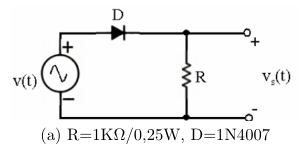
\includegraphics[width=0.8\linewidth]{imagens/circuitos_rel/ca.png}
	\caption{Circuito A\\ retirada do Roteiro do Experimento 1}
	\label{ca}
\end{figure}
\FloatBarrier

O gráfico para a tensão $v \times t$ (em amarelo) e $v_s \times t$ (em verde) é:

- O diodo 'D' está em polarização direta em todos os pontos do gráfico em verde que são maiores que zero. Em todos os que ele é igual a zero, o diodo está em polarização reversa. Como se trata de um diodo retificador, a região de ruptura, que é inclusive evitada, não é atingida nessa experiência!

\begin{figure}[ht!]
	\captionsetup{justification=centering}
	\centering
	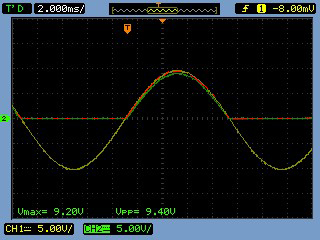
\includegraphics[width=0.8\linewidth]{imagens/circuitos_resp/a01.jpg}
	\caption{Gráfico de tensões pelo tempo - Circuito A\\ Obtido com o auxílio do osciloscópio.}
	\label{a01}
\end{figure}
\FloatBarrier

O Roteiro solicita a característica de transferência $v_0 \times v_I$. Essas grandezas se referem às tensões sobre o resistor (em verde em \ref{a01}) e fornecida pela fonte (em amarelo em \ref{a01}).

O gráfico para a característica de transferência, que pode ser portanto denotado como $V_s \times v$, foi obtido experimentalmente e está representado em \ref{a02}.

O resistor tem a mesma tensão da fonte quando o diodo está em polarização direta. Nos pontos os quais a fonte é negativa, o diodo está em polarização reversa e a tensão no resistor é nula.

\begin{figure}[ht!]
	\captionsetup{justification=centering}
	\centering
	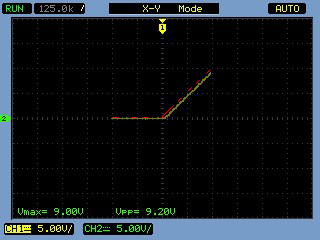
\includegraphics[width=0.8\linewidth]{imagens/circuitos_resp/a02.jpg}
	\caption{Gráfico da característica de transferência do circuito - Circuito A\\ Obtido com o auxílio do osciloscópio}
	\label{a02}
\end{figure}
\FloatBarrier

Podemos então perceber as diferenças entre os gráficos obtidos empiricamente com os esperados de acordo com o desenvolvimento teórico, que adotou um diodo ideal.

No diodo ideal, a superposição dos gráficos $v(t) \times t$ com o $V_s(t) \times t$ fornece uma sinal idêntico no semi-plano positivo do eixo das ordenadas, além da inclinação da reta em $v(t) \times V_s(t)$ se iniciar exatamente na origem.

Entretanto, ao tratar dos diodos reais, observamos a presença de uma pequena queda de tensão $V_D$ no diodo. Desse modo a função $V_s(t)$ estar visualmente um pouco abaixo de $v(t)$ no ponto máximo em \ref{a01} e a reta em \ref{a02} se iniciar um pouco depois da origem nos confirmam as hipóteses e projeções realizadas previamente.

% Experiência 2
\section{Experiência 2}

O circuito montado no laboratório para a experiência 2 é mostrado na figura \ref{cb}.

\begin{figure}[ht!]
	\captionsetup{justification=centering}
	\centering
	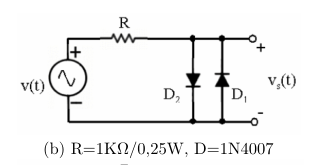
\includegraphics[width=0.8\linewidth]{imagens/circuitos_rel/cb.png}
	\caption{Circuito B\\ retirada do Roteiro do Experimento 1}
	\label{cb}
\end{figure}
\FloatBarrier

Tratando de diodos ideais, a configuração de \ref{cb} nos forneceria uma tensão $V_s(t) = 0\ \forall \ t$. Todavia, a tensão $V_D$ citada anteriormente resulta em um intervalo no qual o diodo em questão não conduz mesmo em polarização direta.

O resultado prático disso é que, para $|v(t)| > V_D$, um dos dois diodos está na região de condução. Entretanto, para $|v(t)| < V_D$, ambos os diodos não permitem passagem de corrente e $V_s(t) = v(t)$.

Desse modo, temos que o diodo 'D1' está em polarização direta na região aproximadamente constante do gráfico em verde da figura \ref{cb} que tem valores maiores que zero. Como o diodo 'D2' tem polarização oposta ao diodo 'D1', ele está em polarização reversa.

Nos valores negativos e aproximadamente constantes do gráfico em verde, o diodo 'D1' tem polarização reversa e, 'D2', direta. Vale lembrar que a tensão de ruptura não é atingida nessa experiência.

O gráfico para a tensão $v \times t$ está em amarelo e $v_s \times t$, em verde.

\begin{figure}[ht!]
	\captionsetup{justification=centering}
	\centering
	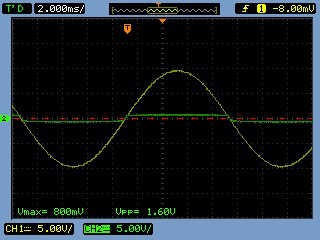
\includegraphics[width=0.8\linewidth]{imagens/circuitos_resp/b01.jpg}
	\caption{Gráfico de tensões pelo tempo - Circuito B\\ Obtido com o auxílio do osciloscópio.}
	\label{b01}
\end{figure}
\FloatBarrier

\begin{figure}[ht!]
	\captionsetup{justification=centering}
	\centering
	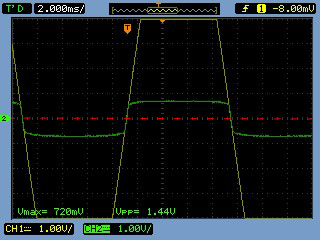
\includegraphics[width=0.8\linewidth]{imagens/circuitos_resp/b01_z.jpg}
	\caption{Zoom do gráfico de tensões pelo tempo - Circuito B\\ Obtido com o auxílio do osciloscópio.}
	\label{b01_z}
\end{figure}
\FloatBarrier

O gráfico para a característica de transferência $v_0 \times v_I$ deste circuito nos ilustra o que é observado em \ref{b01_z}. Existe uma região central onde nenhum dos diodos está na região de condução, dessa forma, a tensão $v_0$ varia aproximadamente linearmente com $v(t)$. Ao atingir a polarização direta que permite que o diodo 1N4007 conduza, seja 'D1' ou 'D2', observamos que $V_s$ se restringe a esse valor $V_D$ independente do valor da fonte.

Como trata-se do mesmo modelo de diodo, percebe-se a simetria do gráfico da figura \ref{b02}. 

\begin{figure}[ht!]
	\captionsetup{justification=centering}
	\centering
	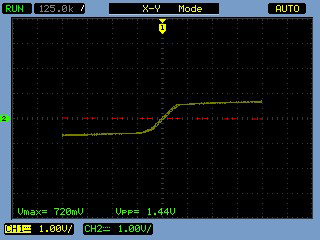
\includegraphics[width=0.8\linewidth]{imagens/circuitos_resp/b02.jpg}
	\caption{Gráfico da característica de transferência do circuito - Circuito B\\ Obtido com o auxílio do osciloscópio.}
	\label{b02}
\end{figure}
\FloatBarrier

% Experiência 3
\section{Experiência 3}

O circuito montado no laboratório para a experiência 3 é mostrado na figura \ref{cc}.

\begin{figure}[ht!]
	\captionsetup{justification=centering}
	\centering
	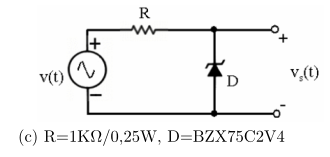
\includegraphics[width=0.8\linewidth]{imagens/circuitos_rel/cc.png}
	\caption{Circuito C\\ retirada do Roteiro do Experimento 1}
	\label{cc}
\end{figure}
\FloatBarrier

O gráfico para a tensão $v \times t$ (em amarelo) e $v_s \times t$ (em verde) obtido está exposto em \ref{c01} e \ref{c01_z}.

\begin{figure}[ht!]
	\captionsetup{justification=centering}
	\centering
	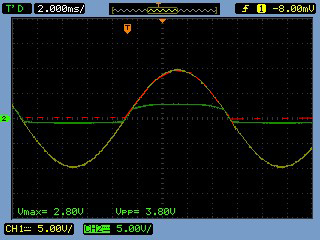
\includegraphics[width=0.8\linewidth]{imagens/circuitos_resp/c01.jpg}
	\caption{Gráfico de tensões pelo tempo - Circuito C\\ Obtido com o auxílio do osciloscópio}
	\label{c01}
\end{figure}
\FloatBarrier

\begin{figure}[ht!]
	\captionsetup{justification=centering}
	\centering
	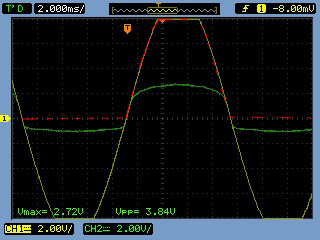
\includegraphics[width=0.8\linewidth]{imagens/circuitos_resp/c01_z.jpg}
	\caption{Zoom do gráfico de tensões pelo tempo - Circuito C\\ Obtido com o auxílio do osciloscópio}
	\label{c01_z}
\end{figure}
\FloatBarrier

Diferentemente da figura \ref{ca}, o diodo em questão sofre polarização direta quando $v(t) < 0$. Para um diodo ideal, teríamos $V_S(t) = v(t)$ na polarização reversa, como ilustrado no gráfico tracejado.

Entretanto, trataremos agora de um diodo Zener. A região de ruptura não foi abordada e nem influenciou os resultados até aqui, entretanto, a funcionalidade do diodo BZX está intimamente atrelada à região de ruptura.

Diferentemente do indicado pelo Roteiro 1, o diodo Zener utilizado no laboratório foi o BZX55C2V4, o qual tem a tensão de ruptura pertencente ao intervalo $2.28<V_Z<2.56$.

Analogamente ao discutido na Experiência 1, o diodo em série com o resistor, quando polarizado diretamente, permitirá que a corrente flua no circuito e a tensão sobre o diodo será teoricamente nula. O diodo Zener, entretanto, também possui um $V_D$ e, como a polarização direta no circuito em \ref{cc} é realizado para valores negativos de $v(t)$, observamos na figura \ref{b01_z} que aparece uma tensão em $V_s(t)$ para tais valores da fonte.

Para $v(t) > 0$, temos que o diodo está em polarização reversa. Todavia, observa-se nos gráficos do osciloscópio que para valores um pouco acima de 2V da fonte, o diodo permite a condução e a tensão sobre tal elemento tende a se manter constante. Nessa situação o diodo atingiu a região de ruptura, prevista pelo valor de $V_Z$ descrito acima.

O gráfico para a característica de transferência $v_0 \times v_I$ está na figura \ref{c02}.

\begin{figure}[ht!]
	\captionsetup{justification=centering}
	\centering
	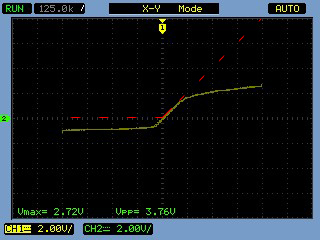
\includegraphics[width=0.8\linewidth]{imagens/circuitos_resp/c02.jpg}
	\caption{Gráfico da característica de transferência do circuito - Circuito C\\ Obtido com o auxílio do osciloscópio}
	\label{c02}
\end{figure}
\FloatBarrier

O gráfico de transferência do circuito em questão, embora tenha similaridade com o da figura \ref{b02}, não é simétrico em relação ao eixo das abscissas. Nesse caso, o valor que $V_S(t)$ se aproxima quando $v(t) \rightarrow - \infty $ está atrelado ao valor $V_D$ do diodo Zener, já o valor que $V_S(t)$ tende quando $v(t) \rightarrow \infty $ é controlado pelo $V_Z$.

% Experiência 4
\section{Experiência 4}

O circuito montado no laboratório para a experiência 4 está ilustrado na figura \ref{cd}.

\begin{figure}[ht!]
	\captionsetup{justification=centering}
	\centering
	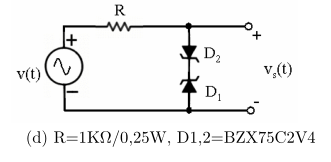
\includegraphics[width=0.8\linewidth]{imagens/circuitos_rel/cd.png}
	\caption{Circuito D\\ retirada do Roteiro do Experimento 1}
	\label{cd}
\end{figure}
\FloatBarrier

O circuito descrito na figura \ref{cc} é bastante semelhante ao atual, porém agora, foi acrescentado um diodo em série com polaridade invertida.

A análise feita anteriormente nos apontou que existem duas possibilidades para que um diodo Zener conduza: ultrapassarmos seus valores característicos de tensão $V_D$ e $V_Z$, os quais tem sinais opostos na análise de circuito.

Para o caso de diodos Zener em polarizações opostas, a corrente flui no circuito quando a tensão no trecho supera $V_Z$ de um e $V_D$ do outro simultaneamente. Na situação em questão, como $V_Z > V_D$, basta que a tensão no ramo seja superior ao valor de $V_Z$.

Para diodos ideais, um dos diodos sempre estará em polarização reversa para todo $t$ e, portanto, a tensão de saída ideal seria a própria tensão da fonte.

\begin{figure}[ht!]
	\captionsetup{justification=centering}
	\centering
	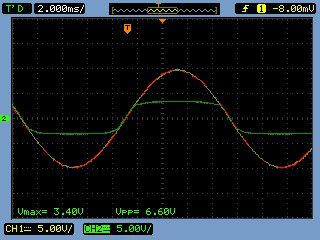
\includegraphics[width=0.8\linewidth]{imagens/circuitos_resp/d01.jpg}
	\caption{Gráfico de tensões pelo tempo - Circuito D\\ Obtido com o auxílio do osciloscópio}
	\label{d01}
\end{figure}
\FloatBarrier

\begin{figure}[ht!]
	\captionsetup{justification=centering}
	\centering
	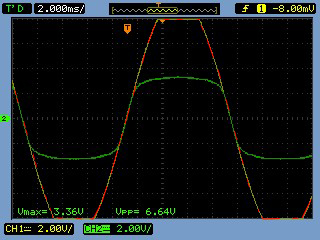
\includegraphics[width=0.8\linewidth]{imagens/circuitos_resp/d01_z.jpg}
	\caption{Zoom do gráfico de tensões pelo tempo - Circuito D\\ Obtido com o auxílio do osciloscópio}
	\label{d01_z}
\end{figure}
\FloatBarrier

As figuras \ref{d01} e \ref{d01_z} nos ilustram que para o circuito atingir uma região de condutividade plena, $v(t) > |V_Z|$. Desse modo, obtemos que o gráfico para a característica de transferência $v_0 \times v_I$ deste circuito é simétrico, assim como o da figura \ref{b02}.

\begin{figure}[ht!]
	\captionsetup{justification=centering}
	\centering
	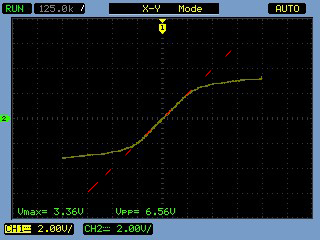
\includegraphics[width=0.8\linewidth]{imagens/circuitos_resp/d02.jpg}
	\caption{Gráfico da característica de transferência do circuito - Circuito D\\ Obtido com o auxílio do osciloscópio}
	\label{d02}
\end{figure}
\FloatBarrier

\section{Questões experimentais e discussão}
\vspace{0.5cm}

\begin{enumerate}
\item As semelhanças e distinções entre os dados empíricos e os previstos teoricamente foram discutidas ao longo das seções anteriores durante a apresentação dos resultados.

\item A medição da tensão $V_S(t)$ sobre o resistor no circuito da figura \ref{ca} é denominado retificador pelo fato do circuito transformar um sinal de entrada fornecido pela fonte, que possui valores positivos e negativos, apenas em seus valores apenas positivos. 

Entretanto, se o sinal de entrada do sistema for positivo e tender ao infinito, $V_s \approx v(t) \approx \infty $, o que evidencia que o circuito não limita a variável de entrada. Além disso, a limitação para regiões negativas é feita de forma completa, ou seja, torna a saída nula para todos os valores negativos de entrada. Isso caracteriza o circuito retificador.

Todavia, se analisarmos a tensão no diodo para valores positivos de $v(t)$, a análise é realizada na região de polarização direta. Por não se tratar de um diodo ideal, a região de condução só é alcançada quando $v(t) = V_D$, dessa forma, temos que, enquanto $v(t) < V_D$, o diodo funcionada como um aberto e a tensão no diodo é igual à tensão da fonte. Porém, quando o diodo passa a conduzir corrente, a tensão medida é limitada em $V_D$.

Se analisarmos os valores negativos de $v(t)$, temos que a tensão no diodo será sempre igual à tensão da fonte.

Por conta das características de limitação apenas para valores positivos de entrada, esse circuito é denominado como limitador simples.

\item Pela descrição acima e baseado nas varáveis de entrada e saída, podemos classificar todos os outros 3 circuitos como limitadores duplos. Perceba que o gráfico de transferência de todos apresenta um limite para valores tanto positivos quanto negativos da entrada $v(t)$.

Esses limites são proporcionados pelos valores de $V_D$ e/ou $V_Z$, dependendo da disposição e dos diodos utilizados. 
\end{enumerate}

% Bibliografia
\bibliography{references}

\begin{thebibliography}{9}

	\bibitem{1} Roteiro do Experimento 1 da Disciplina Laboratório de Eletrônica. Departamento de Engenharia Elétrica - Universidade de Brasília. Brasília, Brasil.

    \bibitem{2} SEDRA; Adel S. e SMITH, Kenneth C. Microeletronics Circuits, 7$^(th)$ Edition. Copyright © 2015, 2010, 2004, 1998 by Oxford University Press;
	
	\bibitem{3}
	KOERICH, Alessandro. \emph{Diodos Eletrônica.} Disponível em: \sloppy
	\url{<http://www.eletrica.ufpr.br/ufpr2/professor/36/TE214/Diodos-Eletronica-P1-four.pdf>}. Acesso em 28 Mar. 2019.
	
	\bibitem{4}
	CIPELLI, Antonio Marco V. \emph{Teoria de Projetos de Circuitos Eletrônicos}, 23º edição – São Paulo: Érica, 2007.

\end{thebibliography}

\end{document}
